% !TEX root = ../main.tex
\chapter{Introduction}
\label{chapter:Introduction}


\section{Motivation}

A worthwhile use of the vast computational resources available in 2018 is on seismic simulations. 

\begin{description}
	\item[SeisSol]
    Simulates earthquakes, specifically, dynamic rupture processes and seismic wave propagation over an unstructured tetrahedral mesh. 

    \item[ADER-DG]
    A numerical method which uses Discontinuous Galerkin discretization in space and ADER discretization in time. It avoids a global system matrix, using local element matrix operations instead.

    \item[Small Sparse Matrix Multiplications]
    The compute kernels resemble the operation shown below, applied recursively. Different sparsity patterns are used, but they are all known at compile time.
\end{description}

\begin{figure}
  \centering
  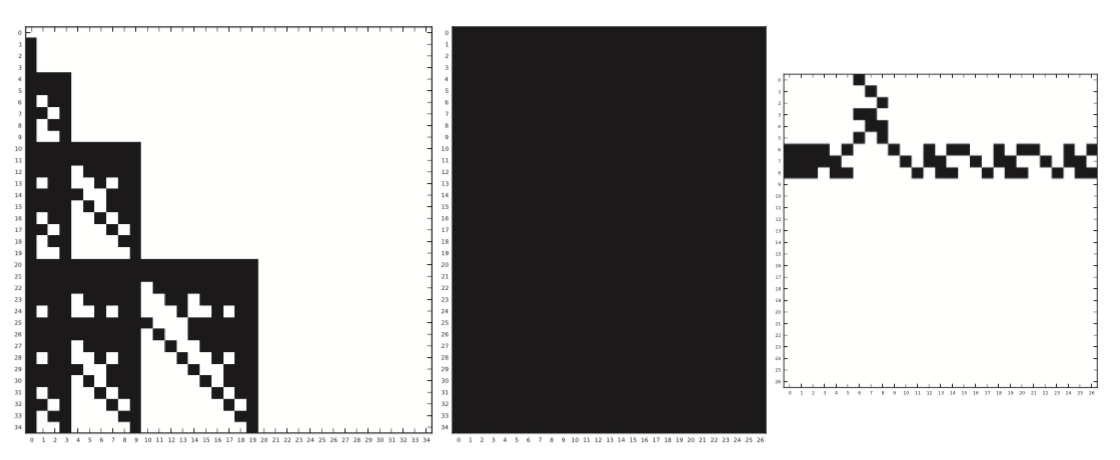
\includegraphics[height=3cm]{images/seissol_visc.png}
  \caption{Common sparsity patterns in SeisSol}
  \label{fig:seissol_star}
\end{figure}

\section{Hardware Constraints}
\label{section:knl}

Although the motivation is straightforward, it is growing increasingly difficult to implement in practice because it is working against current trends in computer architecture. An growing number of the top500 computers are using GPUs or Xeon Phis. This trend is likely to continue because it allows greater parallelism at a lower energy cost. It was desired to run the code on LRZ's CoolMUC3 cluster, which uses Knights Landing.

Knights Landing (KNL) is the second-generation Intel Xeon Phi, a manycore processor that offers greater parallelism and less power consumption in exchange for a slower clock speed. An overview is given by~\cite{Sodani:2016:KLS:2927511.2927563} and a more comprehensive resource is given by~\cite{Jeffers:2016:IXP:3050856}. Unlike its predecessor, Knights Corner, KNL is a host processor rather than a coprocessor, which means that it can run the entire x86-64 instruction set, albeit with a performance penalty for some operations. KNL has two kinds of memory, a high-bandwidth MCDRAM and a high-capacity DDR4. Each processor contains between 64 and 72 cores with 4 hyperthreads per core, resulting in at least 256 logical CPUs. The instruction-level parallelism is similarly impressive, being the first processor to implement the AVX-512 instruction set extensions. These provide 32 vector registers, each of which holds 64 bytes, allowing 8 double-precision floating point numbers to be operated on simultaneously in each \gls{VPU}. Instruction-level performance is further improved by an enhanced \gls{FMA} instruction, which performs $c := c + a*b$ in a single cycle, optionally including a broadcast and a mask. Thus the theoretical peak performance of a single core is given as:

\begin{equation}
  2 \frac{VPUs}{core} \times  = 3 {double TFlop}{sec}
  \label{eq:knl_peak_perf}
\end{equation}

\[\]

This peak performance is in practice merely an upper bound, as it assumes a steady-state throughput of 2 FMAs per cycle. The only algorithms which come close to achieving this are dense matrix multiplication and (to a lesser extent) LU and Cholesky factorization. If the algorithm cannot be vectorized at all, the attainable performance drops by a factor of 8, and if it cannot use the FMA instructions, it drops by a further factor of 2. Hence inherently scalar algorithms perform dramatically worse. This may be a reasonable tradeoff: since scalar algorithms are much more likely to be memory-bound, the extra flops might be wasted. Nevertheless this provides a strong incentive to find creative ways to make the most of the vector registers. 

Another key constraint is cache bandwidth. With only one store unit, KNL can store at most 64B/cycle, corresponding to one vector register. This means that it is essential to accumulate all possible changes to that vector register before storing it. It also makes loop unrolling more important, since this is the only way to amortize the cost of loads and stores.

A number of related bottlenecks encompass the instruction pipeline. Because Knights Landing was derived from the older Silvermont architecture, which was optimized for low power consumption, the instruction pipeline is simpler and narrower. The instruction cache can only provide 16B/cycle, and the decoder can only handle 2 instructions/cycle. Meanwhile, a single \gls{FMA} instruction takes up between 7 and 13 bytes. The most important constraint, however, is that the out-of-order execution pipeline can only issue 2 instructions per cycle. This means that any instruction which is not an FMA \emph{displaces} an FMA, halving the potential computational efficiency of one cycle.


\begin{figure}[tb]
\centering
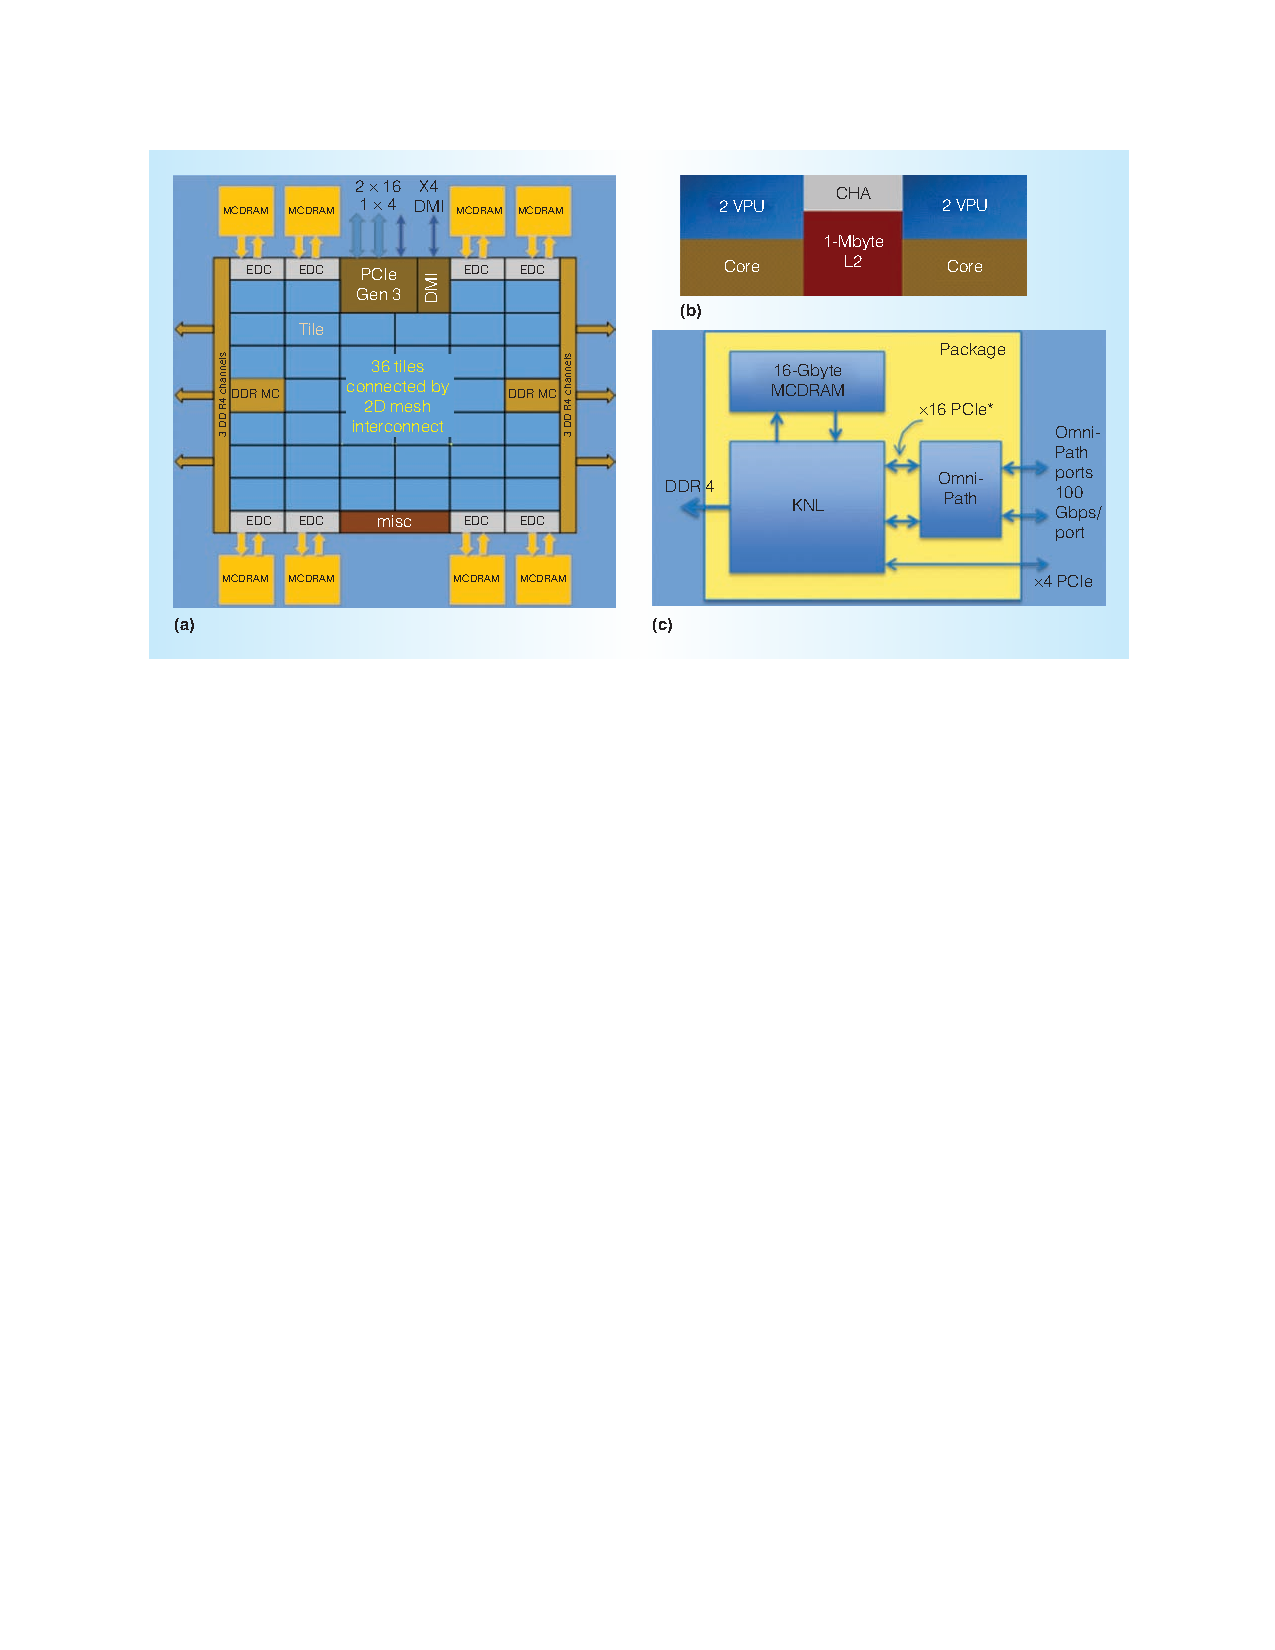
\includegraphics[width=\textwidth]{images/knl_arch.pdf}
\caption{Block diagram of the Knights Landing architecture, taken from~\cite{Sodani:2016:KLS:2927511.2927563}. As shown in (a), each processor is divided into 36 tiles connected in a 2D mesh. As shown in (b), each tile contains 2 cores and a shared L2 cache. Each core has two VPUs and its own L1 caches.}
\end{figure}

\section{Previous approaches}

There is already a substantial amount of effort invested in improving the compute kernels of SeisSol. 

\subsection{CSC sparse multiplication}
  The first approach used standard compressed-sparse-column multiplication. This algorithm goes back to WHOM? . It looks as follows:


  It has the following advantages: It is extremely general, placing no constraints on the matrix size or sparsity. 
  The sparsity pattern itself is known only at runtime. This generality makes it extremely amenable to abstraction, so a 

  Nevertheless, the standard csc multiplication algorithm suffers from several crucial disadvantages: 

\begin{description}
  \item[High memory usage]

  \item[Computational intensity]

  \item[Inability to unroll the innermost loop] This hurts pipeline efficiency.

  \item[Scalar operations]

  The indices are looked up at runtime. Firstly, this requires storing the indices, doubling the amount of memory needed. If only one matrix is sparse, the total number of flops is $2 * m * n * nnz$, with nnz=1/4*n*k, this means that the arithmetic intensity [FLOPs/byte] is 1/8 that of dense matrix multiplication. 
  Although the format lays everything out in memory as efficiently, the algorithm must nevertheless loop over k. The resulting control dependency prevents . The fact that the sparsity pattern is only known at compile time prevents unrolling. 
  A dense-by-sparse algorithm would still benefit from vectorization, but if the 

\end{description}


In the case of SeisSol, the sparsity patterns are derived from the basis functions, which themselves depend mainly on order of accuracy and the choice of viscous damping model. These parameters are all chosen at compile time. Secondly, the problem size is always small: the largest dimension is either 34 (corresponding to ) 56. 

In the case of Knights Landing, these problems are all acerbated. 


  Standard compressed-sparse-column multiplication
    \begin{itemize}
      \item[$+$] Generality.
      \item[$+$] Algorithm uses a (small) constant number of instructions.
      \item[$-$] Index lookups require indirect memory access, causing lots of problems for the execution pipeline.
      \item[$-$] $sparse \times sparse$ is fundamentally scalar. (However, BSR can be vectorized.)
      \item[$-$] Disregards the fact that the sparsity pattern is known at compile time.
    \end{itemize}

  Sparsity pattern unrolled into instruction stream
    \begin{itemize}
    \item[$+$] Index lookups removed completely
    \item[$+$] $dense \times sparse$ case can be vectorized perfectly 
    \item[$-$] Generates one FMA instruction for every nonzero
    \item[$-$] (Implementation) Memory access pattern is suboptimal on KNL
    \item[$-$] (Implementation) Intel compiler struggles to generate efficient assembly
    \end{itemize}

  Current approach: Dense matrix multiplication via libxsmm
    \begin{itemize}
    \item[$+$] Memory access patterns and register blockings optimized for KNL
    \item[$+$] (Implementation) Code generator emits assembly directly 
    \item[$-$] Filling in zero entries wastes both flops and memory bandwidth
    \end{itemize}


  \section{Goals, approach, and design space}

  Each of the existing algorithms discussed in the preceding section encounter different  bottlenecks and constraints. \py{SpGemm} and \py{libxsmm} solve a more general problem than strictly necessary, and Breuer does not use registers Thus there appears to be room to create more complicated algorithms which combine the desirable features of each. The three existing algorithms can be thought of as poles in a barycentric design space, and the aim is to find points in the middle which finesse around the bottlenecks in the corners. One corner has high compute intensity and optimal register usage but wasted flops; another has no wasted flops but many control dependencies and lower compute intensity; the last has no wasted flops and high compute intensity, but poor register usage. The center ought to have decent compute intensity, decent register usage, few control dependencies, and few wasted flops. 


  To keep the scope of this work bounded, we adhere to following assumptions:
  \begin{itemize}
    \item The sparse matrix has a fixed pattern which is known at compile time.
    \item The memory layout of the sparse matrix is not constrained elsewhere.
    \item All matrices fit in the L2 cache: $(mn + mk + kn)\cdot 8 \leq 1e6$
  \end{itemize}

  Within this framework, we consider variations of the following:
  \begin{itemize}
    \item Modifications of the sparsity pattern
    \item Modifications of the control flow
    \item The memory layout of the sparse matrix
    \item The block sizes, if a block decomposition is used
    \item The ordering and unrolling of the loop nest
  \end{itemize}


Although interesting, we disregard prefetching, instruction alignment, and register assignment. 

The goal of this work is to find algorithms which might outperform the status quo, and write a code generator which will emit an instance of each relevant algorithm for a given problem. The generator should be able to handle different matrix sizes, number of nonzeros, and sparsity patterns, while staying within the aforementioned assumptions. 

Once implemented, the generators can be tested -- using the actual SeisSol matrices -- to determine if they yield a speedup. Equally interesting is exploring the algorithm's problem space constraints. Using both the observed and estimated performance, we can address the questions ``which problems can this algorithm handle efficiently?'' and ``which algorithm is best for a given problem?''. 

Each algorithm requires additional tuning parameters, and the effect of these should also be estimated and tested, addressing the question ``which parameters yield the best kernel for a given problem?''. If possible, heuristics should be given in order to choose these parameters automatically.

   
\section{Roadmap} 
  This work is broken down as follows. Chapter 2 lays out the fundamental concepts and terminology. Chapter 3 covers a progression of different dense-by-sparse kernels in depth, and discusses strategies for sparse-by-dense and tensor kernels which might benefit from a similar treatment. Chapter 4 discusses the design of the code generator, and provides a brief manual illustrating its use. Chapter 5 walks through some experiment results, attempting to discern performance and scaling characteristics. Finally, Chapter 6 wraps everything up.










